\chapter{Экспериментальная часть}

В данном разделе описаны проведённые замеры и представлены результаты исследования. Также будут уточнены характеристики устройства, на котором проводились замеры.

\section{Технические характеристики}
Технические характеристики устройства, на котором выполнялись замеры времени выполнения \cite{web_item5}:
\begin{itemize}
	\item операционная система macOS Monterey 12.4;
	\item 8 ГБ оперативной памяти;
	\item процессор Apple M2 (базовая частота~---~2400 МГц, но поддержка технологии Turbo Boost позволяет достигать частоты в 3500 МГц \cite{web_item10}).
\end{itemize}

\section{Измерение времени выполнения реализаций алгоритма}
Время работы алгоритма обратной трассировки лучей замерялось с помощью класса $std::chrono::system\_clock$ \cite{web_item11}, который представляет реальное время. В исследуемых изображениях растр имеет одинаковое количество пикселей в обоих плоских измерениях.

Результаты замеров времени выполнения (в мс) приведены в таблице \ref{table:time1}. замеры проводились до значения количества выделяемых потоков равного 32, так как уже на этом значении происходит замедление работы алгоритма. Количество потоков равное нулю означает, что замер проведён для однопоточной реализации, что отличается от столбца, соответствующего одному потоку, так как для последнего подразумевается именно переключение на новый поток. На рисунке \ref{img:graph1} приведён график, отображающий зависимость времени работы реализации алгоритма от количества выделяемых потоков. Выполнялась визуализация сцены из 3 объектов, представленной на рис. \ref{img:p2}. В замерах использовались изображения размером от $128 \times 128$ пикселов до $512 \times 512$ пикселов.

\begin{table}[H]
	\begin{center}
		\caption{\label{table:time1} Таблица времени выполнения реализации алгоритма (мс)}
		\begin{tabular}{
    |S[table-format=4.0]
    |S[table-format=4.3]
    |S[table-format=4.3]
    |S[table-format=4.3]
    |S[table-format=4.3]
    |S[table-format=4.3]
    |S[table-format=4.3]
    |S[table-format=4.3]|
    }
			\hline
			{\specialcell{Размер\\изображения\\(в пикселях)}} & \multicolumn{7}{c|}{Количество потоков}\\ 
			\cline{2-8}
			&   {0}&{1}&{2}&{4}&{8}&{18}&{32}\\ 
		
			\hline
			128 & 187.727 & 189.169 & 96.128 & 54.11 & 33.404 & 35.011 & 63.605\\ \hline
			256 & 763.037 & 774.614 & 390.659 & 203.641 & 122.011 & 124.56  & 231.414\\ \hline
			384 & 1732.54 & 1728.67 & 886.806 & 466.111 & 298.466 & 299.978 & 508.959\\ \hline
			512 & 8140.94 & 8145.62 & 4146.27 & 3424.31 & 2958.07 & 2023.53 & 2375.9\\ \hline
			
		\end{tabular}
	\end{center}
\end{table}

\noindent
\begin{table}[h!]
  \centering
  \begin{tabular}{p{1\linewidth}}
    \centering
    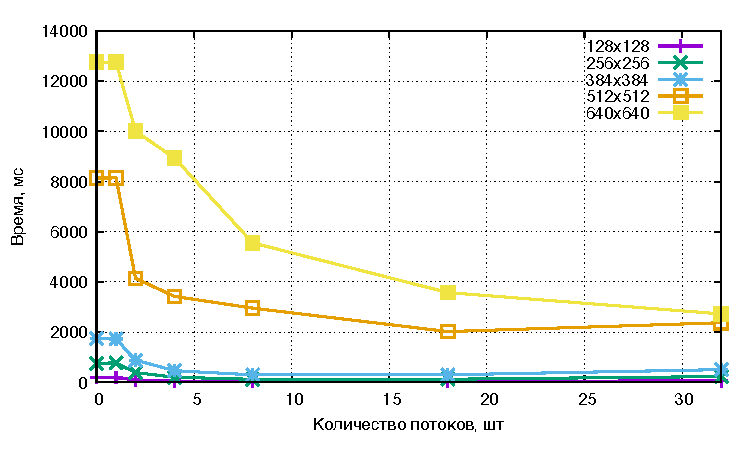
\includegraphics[width=1\linewidth]{../images/time.pdf}
    \captionof{figure}{Зависимость времени работы алгоритма от количества выделяемых потоков}
    \label{img:graph1}
  \end{tabular}
\end{table}

\newpage